% Options for packages loaded elsewhere
% Options for packages loaded elsewhere
\PassOptionsToPackage{unicode}{hyperref}
\PassOptionsToPackage{hyphens}{url}
%
\documentclass[
  ignorenonframetext,
  aspectratio=169,
]{beamer}
\newif\ifbibliography
\usepackage{pgfpages}
\setbeamertemplate{caption}[numbered]
\setbeamertemplate{caption label separator}{: }
\setbeamercolor{caption name}{fg=normal text.fg}
\beamertemplatenavigationsymbolsempty
% remove section numbering
\setbeamertemplate{part page}{
  \centering
  \begin{beamercolorbox}[sep=16pt,center]{part title}
    \usebeamerfont{part title}\insertpart\par
  \end{beamercolorbox}
}
\setbeamertemplate{section page}{
  \centering
  \begin{beamercolorbox}[sep=12pt,center]{section title}
    \usebeamerfont{section title}\insertsection\par
  \end{beamercolorbox}
}
\setbeamertemplate{subsection page}{
  \centering
  \begin{beamercolorbox}[sep=8pt,center]{subsection title}
    \usebeamerfont{subsection title}\insertsubsection\par
  \end{beamercolorbox}
}
% Prevent slide breaks in the middle of a paragraph
\widowpenalties 1 10000
\raggedbottom
\AtBeginPart{
  \frame{\partpage}
}
\AtBeginSection{
  \ifbibliography
  \else
    \frame{\sectionpage}
  \fi
}
\AtBeginSubsection{
  \frame{\subsectionpage}
}
\usepackage{iftex}
\ifPDFTeX
  \usepackage[T1]{fontenc}
  \usepackage[utf8]{inputenc}
  \usepackage{textcomp} % provide euro and other symbols
\else % if luatex or xetex
  \usepackage{unicode-math} % this also loads fontspec
  \defaultfontfeatures{Scale=MatchLowercase}
  \defaultfontfeatures[\rmfamily]{Ligatures=TeX,Scale=1}
\fi
\usepackage{lmodern}

\ifPDFTeX\else
  % xetex/luatex font selection
\fi
% Use upquote if available, for straight quotes in verbatim environments
\IfFileExists{upquote.sty}{\usepackage{upquote}}{}
\IfFileExists{microtype.sty}{% use microtype if available
  \usepackage[]{microtype}
  \UseMicrotypeSet[protrusion]{basicmath} % disable protrusion for tt fonts
}{}
\makeatletter
\@ifundefined{KOMAClassName}{% if non-KOMA class
  \IfFileExists{parskip.sty}{%
    \usepackage{parskip}
  }{% else
    \setlength{\parindent}{0pt}
    \setlength{\parskip}{6pt plus 2pt minus 1pt}}
}{% if KOMA class
  \KOMAoptions{parskip=half}}
\makeatother


\usepackage{longtable,booktabs,array}
\usepackage{calc} % for calculating minipage widths
\usepackage{caption}
% Make caption package work with longtable
\makeatletter
\def\fnum@table{\tablename~\thetable}
\makeatother
\usepackage{graphicx}
\makeatletter
\newsavebox\pandoc@box
\newcommand*\pandocbounded[1]{% scales image to fit in text height/width
  \sbox\pandoc@box{#1}%
  \Gscale@div\@tempa{\textheight}{\dimexpr\ht\pandoc@box+\dp\pandoc@box\relax}%
  \Gscale@div\@tempb{\linewidth}{\wd\pandoc@box}%
  \ifdim\@tempb\p@<\@tempa\p@\let\@tempa\@tempb\fi% select the smaller of both
  \ifdim\@tempa\p@<\p@\scalebox{\@tempa}{\usebox\pandoc@box}%
  \else\usebox{\pandoc@box}%
  \fi%
}
% Set default figure placement to htbp
\def\fps@figure{htbp}
\makeatother





\setlength{\emergencystretch}{3em} % prevent overfull lines

\providecommand{\tightlist}{%
  \setlength{\itemsep}{0pt}\setlength{\parskip}{0pt}}



 


% ============================================================
%  UNL Combined Style
%  Combines: nav-bar (pic1) + title page (pic2) + footer (pic3)
% ============================================================

\usepackage{xcolor}

% ── UNL Brand Colors ────────────────────────────────────────
\definecolor{unlscarlet}{HTML}{D00000}
\definecolor{unlcream}{HTML}{F2EFE8}
\definecolor{unlgray}{HTML}{5C5C5C}

% ── Base theme: no default decorations ─────────────────────
\usetheme{default}
\usecolortheme{default}
\setbeamertemplate{navigation symbols}{}

% ── TOP navigation bar with section tabs + progress dots ───
%    This is the key feature from Screenshot 1
\useoutertheme[subsection=false]{miniframes}
\setbeamercolor{section in head/foot}{bg=unlscarlet, fg=white}
\setbeamerfont{section in head/foot}{size=\tiny, series=\bfseries}
% Dot colors: filled = visited, empty = upcoming
\setbeamercolor{mini frame}{fg=white, bg=unlscarlet}
\setbeamercolor{mini frame in current section}{fg=white, bg=unlscarlet}
\setbeamercolor{mini frame in other section}{fg=unlscarlet!40, bg=white}

% ── Frametitle: scarlet bar, white bold text (pic 1 & 3) ───
\setbeamercolor{frametitle}{bg=unlscarlet, fg=white}
\setbeamerfont{frametitle}{size=\normalsize, series=\bfseries}
\setbeamertemplate{frametitle}{%
  \nointerlineskip
  \begin{beamercolorbox}[wd=\paperwidth, ht=0.6cm, dp=0.15cm,
      leftskip=0.5cm]{frametitle}
    \usebeamerfont{frametitle}\insertframetitle
  \end{beamercolorbox}
}

% ── Structure / bullet color ────────────────────────────────
\setbeamercolor{structure}{fg=unlscarlet}
\setbeamercolor{itemize item}{fg=unlscarlet}
\setbeamercolor{itemize subitem}{fg=unlscarlet}
\setbeamertemplate{itemize item}{\textbullet}
\setbeamertemplate{itemize subitem}{--}

% ── Block colors ────────────────────────────────────────────
\setbeamercolor{block title}{bg=unlscarlet, fg=white}
\setbeamercolor{block body}{bg=unlcream, fg=black}

% ── Title page: scarlet text, centered, multi-line (pic 2) ─
\setbeamercolor{title}{fg=unlscarlet, bg=white}
\setbeamercolor{subtitle}{fg=unlscarlet, bg=white}
\setbeamerfont{title}{size=\large, series=\bfseries}
\setbeamerfont{subtitle}{size=\normalsize, series=\normalfont}
\setbeamerfont{author}{size=\normalsize, series=\bfseries}
\setbeamerfont{institute}{size=\small, series=\normalfont}
\setbeamerfont{date}{size=\small}

\setbeamertemplate{title page}{%
  \vfill
  \begin{center}
    {\usebeamerfont{title}\usebeamercolor[fg]{title}\inserttitle}
    \ifx\insertsubtitle\@empty\else
      \\[0.35em]
      {\usebeamerfont{subtitle}\usebeamercolor[fg]{subtitle}\insertsubtitle}
    \fi
    \\[0.6em]
    \textcolor{unlscarlet}{\rule{0.55\textwidth}{0.5pt}}
    \\[0.55em]
    {\usebeamerfont{author}\insertauthor}
    \\[0.3em]
    {\usebeamerfont{institute}\insertinstitute}
    \\[0.25em]
    {\usebeamerfont{date}\insertdate}
  \end{center}
  \vfill
}

% ── Footer: cream bar, short title | author, slide N/Total ─
%    Matches Screenshot 3 footer exactly
\setbeamertemplate{footline}{%
  \leavevmode
  \begin{beamercolorbox}[%
      wd=\paperwidth, ht=0.5cm, dp=0.2cm,
      leftskip=0.5cm, rightskip=0.5cm]{block body}%  uses cream bg
    \textcolor{unlgray}{\small%
      \textbf{\insertshorttitle}\ \textbar\ \insertshortauthor
      \hfill
      \insertframenumber\,/\,\inserttotalframenumber
    }%
  \end{beamercolorbox}%
}

% ── Two-column helper (like \UNLtwocol in pic 3) ───────────
\newcommand{\twocol}[2]{%
  \begin{columns}[T]
    \begin{column}{0.47\textwidth}#1\end{column}
    \hfill
    \begin{column}{0.47\textwidth}#2\end{column}
  \end{columns}%
}

% ── Highlight / Key point box (like pic 3 bottom box) ──────
\newcommand{\keypoint}[1]{%
  \vspace{0.4em}
  \begin{beamercolorbox}[%
      rounded=false, shadow=false,
      wd=\textwidth, dp=0.25cm, ht=0.4cm,
      leftskip=0.4cm, rightskip=0.4cm]{block body}
    \textbf{Key point:}\ #1
  \end{beamercolorbox}%
}

% ---------- Title page ----------
\setbeamertemplate{title page}{
  \begin{centering}
    \vspace{0.7cm}

    {\usebeamerfont{title}\usebeamercolor[fg]{title}\inserttitle\par}
    \vspace{0.2cm}

    {\usebeamerfont{subtitle}\usebeamercolor[fg]{subtitle}\insertsubtitle\par}
    \vspace{0.5cm}

    {\Large\bfseries \insertauthor \par}
    \vspace{0.08cm}

    {\small \insertinstitute \par}
    \vspace{0.04cm}



    \vfill
  \end{centering}
}
\makeatletter
\@ifpackageloaded{caption}{}{\usepackage{caption}}
\AtBeginDocument{%
\ifdefined\contentsname
  \renewcommand*\contentsname{Table of contents}
\else
  \newcommand\contentsname{Table of contents}
\fi
\ifdefined\listfigurename
  \renewcommand*\listfigurename{List of Figures}
\else
  \newcommand\listfigurename{List of Figures}
\fi
\ifdefined\listtablename
  \renewcommand*\listtablename{List of Tables}
\else
  \newcommand\listtablename{List of Tables}
\fi
\ifdefined\figurename
  \renewcommand*\figurename{Figure}
\else
  \newcommand\figurename{Figure}
\fi
\ifdefined\tablename
  \renewcommand*\tablename{Table}
\else
  \newcommand\tablename{Table}
\fi
}
\@ifpackageloaded{float}{}{\usepackage{float}}
\floatstyle{ruled}
\@ifundefined{c@chapter}{\newfloat{codelisting}{h}{lop}}{\newfloat{codelisting}{h}{lop}[chapter]}
\floatname{codelisting}{Listing}
\newcommand*\listoflistings{\listof{codelisting}{List of Listings}}
\makeatother
\makeatletter
\makeatother
\makeatletter
\@ifpackageloaded{caption}{}{\usepackage{caption}}
\@ifpackageloaded{subcaption}{}{\usepackage{subcaption}}
\makeatother

\usepackage{bookmark}
\IfFileExists{xurl.sty}{\usepackage{xurl}}{} % add URL line breaks if available
\urlstyle{same}
\hypersetup{
  pdftitle={Change-Point Detection in Logistic and Epidemic Models: Computational and Inferential Consequences},
  pdfauthor={Maksuda Toma, Dinuwanthi Liyanage, Ovini Kariyawasam},
  hidelinks,
  pdfcreator={LaTeX via pandoc}}


\title[Computational Statistics]{Change-Point Detection in Logistic and
Epidemic Models: Computational and Inferential Consequences}
\author[UNL]{Maksuda Toma, Dinuwanthi Liyanage, Ovini Kariyawasam}
\date{}
\institute{Department of Statistics, University of Nebraska--Lincoln}

\begin{document}
\frame{\titlepage}


\begin{frame}{Content}
\phantomsection\label{content}
\begin{itemize}
\tightlist
\item
  Introduction
\item
  Motivation and Objective
\item
  Logistic Growth Model
\item
  Bayesian Approach for Logistic Model
\item
  SIR Model
\item
  Bayesian Approach for SIR Model
\item
  Practical Recommendations
\item
  Discussion and Conclusion
\end{itemize}
\end{frame}

\section{Introduction}\label{introduction}

\begin{frame}{Introduction}
\phantomsection\label{introduction-1}
\begin{itemize}
\tightlist
\item
  Nonlinear growth processes arise in many scientific fields:

  \begin{itemize}
  \tightlist
  \item
    ecology, population dynamics, epidemiology
  \end{itemize}
\item
  Common modeling frameworks:

  \begin{itemize}
  \tightlist
  \item
    logistic growth \(\rightarrow\) population expansion with limits
  \item
    SIR models \(\rightarrow\) infectious disease spread
  \end{itemize}
\item
  Real-world systems are rarely stable over time:

  \begin{itemize}
  \tightlist
  \item
    environmental changes
  \item
    policy interventions
  \item
    behavioral shifts
  \end{itemize}
\item
  These can alter key model parameters and create different regimes.
\end{itemize}
\end{frame}

\begin{frame}{Motivation and Objective}
\phantomsection\label{motivation-and-objective}
\begin{itemize}
\tightlist
\item
  We use \textbf{change-point models} to allow parameters to shift at an
  unknown time point.
\item
  Main questions:

  \begin{itemize}
  \tightlist
  \item
    When does the change occur?
  \item
    How do parameter values differ before and after the change?
  \item
    What happens if the change is ignored?
  \end{itemize}
\item
  Challenges:

  \begin{itemize}
  \tightlist
  \item
    nonlinear models lack closed-form solutions
  \item
    change-point introduces mixed discrete and continuous parameters
  \item
    SIR models require solving differential equations
  \end{itemize}
\item
  Our strategy:

  \begin{itemize}
  \tightlist
  \item
    start with logistic growth as a baseline
  \item
    extend to SIR for a more mechanistic setting
  \item
    compare frequentist and Bayesian inference
  \end{itemize}
\end{itemize}
\end{frame}

\section{Model}\label{model}

\begin{frame}{Logistic Growth Model}
\phantomsection\label{logistic-growth-model}
\textbf{Baseline model (no change-point)}

\[
y_i = f(t_i;\theta) + \varepsilon_i, \qquad \varepsilon_i \sim N(0,\sigma^2)
\]

with mean function

\[
f(t_i;\theta) = \frac{K}{1 + \exp\{-r(t_i - t_0)\}}.
\]

\begin{itemize}
\tightlist
\item
  Growth starts slowly, increases rapidly, and then levels off at a
  maximum.
\end{itemize}
\end{frame}

\begin{frame}{Logistic Change-Point Model}
\phantomsection\label{logistic-change-point-model}
\begin{itemize}
\tightlist
\item
  Real systems may experience a shift in growth behavior over time.
\item
  Introduce a change-point \(\tau\) so the growth rate changes at an
  unknown time.
\end{itemize}

\[
f(t_i;\theta)=
\begin{cases}
\dfrac{K}{1+\exp\{-r_1(t_i-t_0)\}}, & t_i \le \tau, \\
\dfrac{K}{1+\exp\{-r_2(t_i-t_0)\}}, & t_i > \tau.
\end{cases}
\]

\begin{itemize}
\tightlist
\item
  Before \(\tau\): growth rate \(r_1\)
\item
  After \(\tau\): growth rate \(r_2\)
\end{itemize}
\end{frame}

\begin{frame}{Parameters and Assumptions}
\phantomsection\label{parameters-and-assumptions}
\textbf{Parameters}

\begin{itemize}
\tightlist
\item
  \(K\): carrying capacity
\item
  \(t_0\): inflection point
\item
  \(r_1, r_2\): growth rates
\item
  \(\tau\): change-point
\item
  \(\sigma^2\): error variance
\end{itemize}

\textbf{Assumptions}

\begin{itemize}
\tightlist
\item
  Logistic growth holds within each regime.
\item
  A single change-point exists.
\item
  Parameters are constant within each segment.
\item
  Errors are independent with constant variance.
\item
  The change is large enough for identifiability.
\end{itemize}
\end{frame}

\begin{frame}[fragile]{Frequentist Estimation: Logistic Model}
\phantomsection\label{frequentist-estimation-logistic-model}
\begin{itemize}
\tightlist
\item
  Parameters estimated using \textbf{maximum likelihood estimation
  (MLE)}.
\item
  Under Gaussian errors, this is equivalent to minimizing the negative
  log-likelihood.
\item
  Optimization in R:

  \begin{itemize}
  \tightlist
  \item
    \texttt{optim()}
  \item
    \texttt{L-BFGS-B} algorithm
  \end{itemize}
\item
  No change-point model:

  \begin{itemize}
  \tightlist
  \item
    directly estimate \((K, r, t_0, \sigma)\)
  \end{itemize}
\item
  Change-point model:

  \begin{itemize}
  \tightlist
  \item
    treat \(\tau\) as discrete
  \item
    use a grid search over candidate values of \(\tau\)
  \item
    for each candidate, optimize the remaining parameters
  \item
    choose the value of \(\tau\) minimizing the negative log-likelihood
  \end{itemize}
\item
  Model comparison is based on AIC.
\end{itemize}
\end{frame}

\begin{frame}{Logistic Simulation Study}
\phantomsection\label{logistic-simulation-study}
\begin{itemize}
\tightlist
\item
  Goal: assess performance of the change-point logistic model
\item
  Data generated from a logistic model with a true change-point
\item
  Setup:

  \begin{itemize}
  \tightlist
  \item
    sample size \(n = 60\)
  \item
    true parameters:

    \begin{itemize}
    \tightlist
    \item
      \(K = 100\)
    \item
      \(t_0 = 25\)
    \item
      \(r_1 = 0.22\)
    \item
      \(r_2 = 0.06\)
    \item
      \(\tau = 30\)
    \end{itemize}
  \end{itemize}
\item
  Procedure:

  \begin{itemize}
  \tightlist
  \item
    simulate dataset
  \item
    fit both no-change and change-point models
  \item
    repeat for 100 replications
  \end{itemize}
\item
  Metrics:

  \begin{itemize}
  \tightlist
  \item
    bias
  \item
    RMSE
  \item
    change-point detection accuracy
  \item
    AIC-based model selection
  \end{itemize}
\end{itemize}
\end{frame}

\begin{frame}{Logistic Simulation Results}
\phantomsection\label{logistic-simulation-results}
\begin{longtable}[]{@{}lrrr@{}}
\toprule\noalign{}
Parameter & True Value & Mean Estimate & RMSE \\
\midrule\noalign{}
\endhead
\(K\) & 100.00 & 100.45 & 6.58 \\
\(r_1\) & 0.22 & 0.221 & 0.013 \\
\(r_2\) & 0.06 & 0.061 & 0.012 \\
\(t_0\) & 25.00 & 25.05 & 0.68 \\
\(\tau\) & 30.00 & 29.93 & 0.52 \\
\bottomrule\noalign{}
\end{longtable}

\textbf{Takeaway:} estimates are close to the true values, with low
variability overall.
\end{frame}

\begin{frame}{Logistic Model: Key Insights}
\phantomsection\label{logistic-model-key-insights}
\begin{itemize}
\tightlist
\item
  \textbf{Accuracy:} negligible bias for most parameters
\item
  Slight positive bias in \(K\), but small relative to its scale
\item
  \textbf{Precision:} low RMSE for most parameters
\item
  Higher RMSE for \(K\) reflects difficulty in estimating the plateau
  level
\item
  \textbf{Change-point detection:} 98\% of \(\hat\tau\) values fall
  within \(\pm 2\) of the true value
\item
  \textbf{Model selection:} the change-point model is preferred in 100\%
  of simulations by AIC
\end{itemize}
\end{frame}

\begin{frame}{Parametric Bootstrap: Logistic Model}
\phantomsection\label{parametric-bootstrap-logistic-model}
\begin{itemize}
\tightlist
\item
  Goal: quantify uncertainty in frequentist estimates
\item
  Bootstrap based on the fitted change-point model
\item
  200 bootstrap replications
\end{itemize}

\begin{longtable}[]{@{}ll@{}}
\toprule\noalign{}
Parameter & 95\% CI \\
\midrule\noalign{}
\endhead
\(\tau\) & \((28.98, 31.00)\) \\
\(K\) & \((92.18, 115.87)\) \\
\(r_1\) & \((0.187, 0.240)\) \\
\(r_2\) & \((0.035, 0.083)\) \\
\(t_0\) & \((24.46, 26.90)\) \\
\(\sigma\) & \((2.29, 3.44)\) \\
\bottomrule\noalign{}
\end{longtable}

\begin{itemize}
\tightlist
\item
  \(\tau\): narrow CI, centered near the true value
\item
  \(K\): widest interval
\item
  \(r_1\) estimated more precisely than \(r_2\)
\item
  Overall: bootstrap confirms stable and reliable frequentist inference
\end{itemize}
\end{frame}

\begin{frame}{Bayesian Approach: Logistic Model}
\phantomsection\label{bayesian-approach-logistic-model}
\begin{itemize}
\tightlist
\item
  Advantages:

  \begin{itemize}
  \tightlist
  \item
    captures joint uncertainty across all parameters
  \item
    avoids reliance on asymptotic approximations
  \item
    naturally handles uncertainty in \(\tau\)
  \end{itemize}
\item
  Weakly informative priors chosen to match MLE bounds
\item
  With \(n = 60\), the likelihood dominates the priors
\end{itemize}

\textbf{MCMC setup}

\begin{itemize}
\tightlist
\item
  Metropolis-within-Gibbs sampler
\item
  Continuous parameters: Gaussian random-walk proposals
\item
  \(\tau\): discrete random-walk proposal
\item
  Tuning target: acceptance rate \(0.20\)--\(0.50\)
\item
  Run length:

  \begin{itemize}
  \tightlist
  \item
    50,000 iterations
  \item
    5,000 burn-in
  \item
    thinning by 10
  \item
    4,500 posterior samples retained
  \end{itemize}
\end{itemize}
\end{frame}

\begin{frame}{MCMC Tuning and Diagnostics}
\phantomsection\label{mcmc-tuning-and-diagnostics}
\begin{longtable}[]{@{}lrr@{}}
\toprule\noalign{}
Parameter & Proposal SD & Acceptance Rate \\
\midrule\noalign{}
\endhead
\(K\) & 4.0 & 0.213 \\
\(r_1\) & 0.025 & 0.347 \\
\(r_2\) & 0.008 & 0.223 \\
\(t_0\) & 1.0 & 0.200 \\
\(\sigma\) & 0.8 & 0.378 \\
\(\tau\) & \(\pm\{1,2\}\) & 0.016 \\
\bottomrule\noalign{}
\end{longtable}

\begin{itemize}
\tightlist
\item
  Continuous-parameter acceptance rates fall in the target range.
\item
  Low acceptance for \(\tau\) is expected because of strong posterior
  concentration.
\item
  ESS and ACF show:

  \begin{itemize}
  \tightlist
  \item
    high efficiency for \(\sigma\) and \(\tau\)
  \item
    slower mixing for \(K, r_1, r_2, t_0\) due to parameter dependence
  \end{itemize}
\item
  Trace plots are stationary and show adequate convergence.
\end{itemize}
\end{frame}

\begin{frame}{Logistic MCMC Diagnostics: Trace and ACF}
\phantomsection\label{logistic-mcmc-diagnostics-trace-and-acf}
\begin{columns}[T]
\begin{column}{0.5\linewidth}
\begin{figure}[H]

{\centering 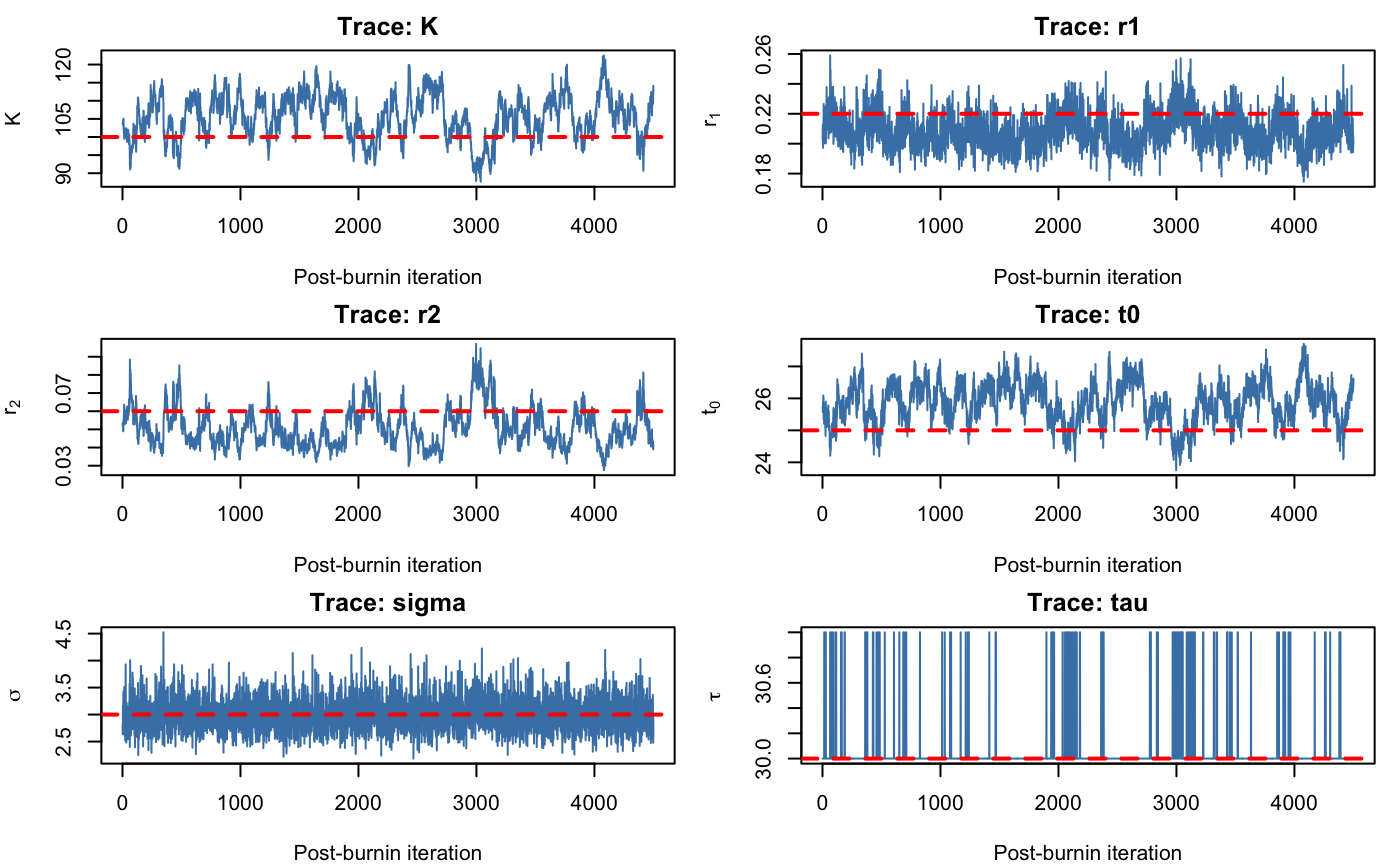
\includegraphics[width=1\linewidth,height=\textheight,keepaspectratio]{trace.png}

}

\caption{Trace plots after burn-in.}

\end{figure}%
\end{column}

\begin{column}{0.5\linewidth}
\begin{figure}[H]

{\centering 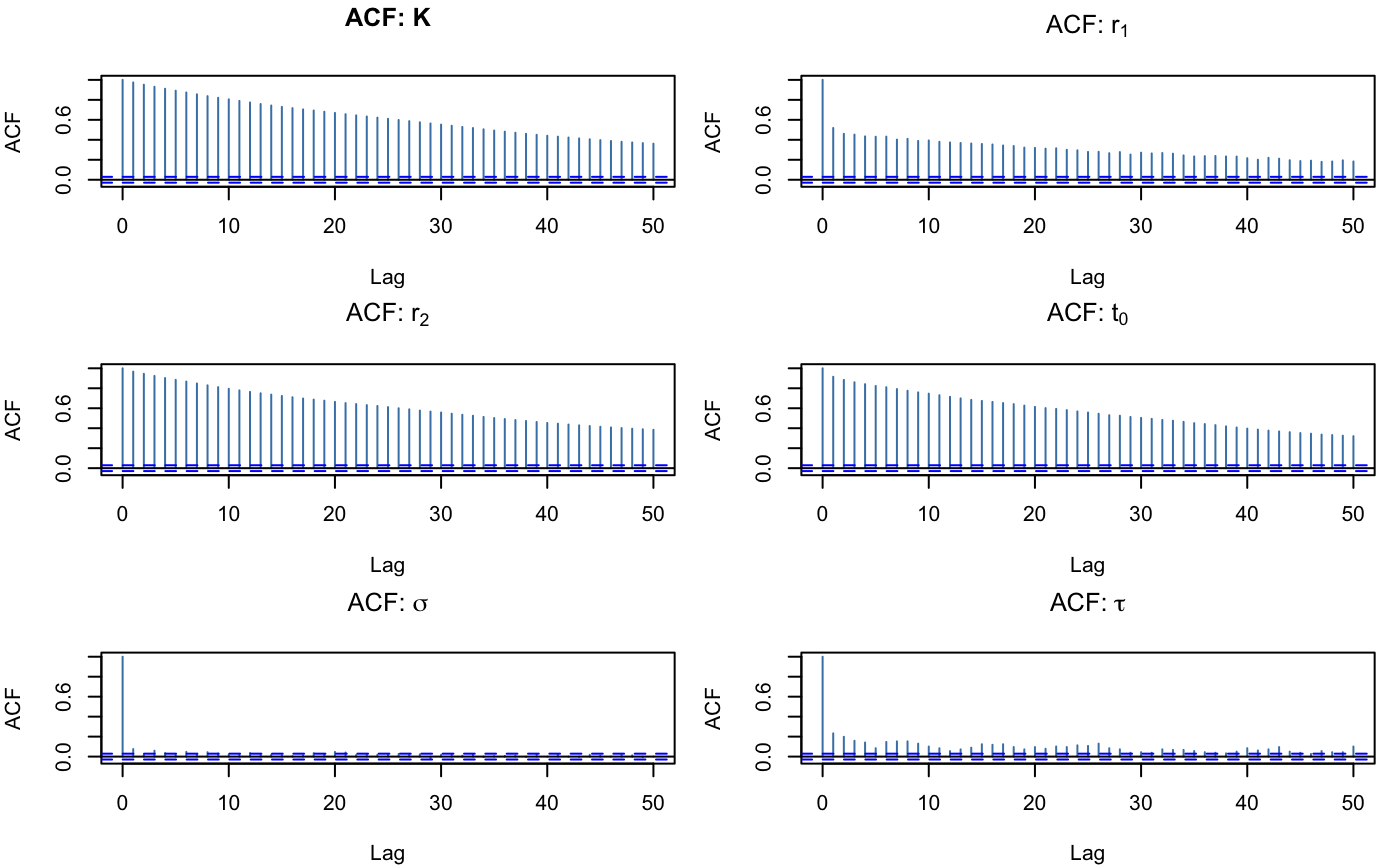
\includegraphics[width=1\linewidth,height=\textheight,keepaspectratio]{ACF.png}

}

\caption{ACF plots after thinning.}

\end{figure}%
\end{column}
\end{columns}

\begin{itemize}
\tightlist
\item
  Trace plots show stationarity and no drift.
\item
  \(\sigma\) and \(\tau\) mix well; \(K\), \(r_1\), \(r_2\), and \(t_0\)
  mix more slowly.
\item
  Diagnostics support convergence.
\end{itemize}
\end{frame}

\begin{frame}{Posterior Summary: Logistic Model}
\phantomsection\label{posterior-summary-logistic-model}
\begin{longtable}[]{@{}lrrrl@{}}
\toprule\noalign{}
Parameter & True Value & Post. Mean & Post. Median & 95\% CI \\
\midrule\noalign{}
\endhead
\(\tau\) & 30.00 & 30.05 & 30.00 & \((30, 31)\) \\
\(K\) & 100.00 & 104.52 & 104.10 & \((93.05, 115.39)\) \\
\(r_1\) & 0.220 & 0.213 & 0.213 & \((0.191, 0.235)\) \\
\(r_2\) & 0.060 & 0.054 & 0.053 & \((0.037, 0.077)\) \\
\(t_0\) & 25.00 & 25.76 & 25.80 & \((24.57, 26.88)\) \\
\(\sigma\) & 3.000 & 3.024 & 2.999 & \((2.490, 3.648)\) \\
\bottomrule\noalign{}
\end{longtable}

\begin{itemize}
\tightlist
\item
  All true values are well recovered.
\item
  \(\tau\) is estimated very precisely.
\item
  \(K\) has the largest uncertainty.
\end{itemize}
\end{frame}

\begin{frame}{Bootstrap vs Bayesian: Logistic Model}
\phantomsection\label{bootstrap-vs-bayesian-logistic-model}
\begin{columns}[T]
\begin{column}{0.55\linewidth}
\begin{figure}[H]

{\centering 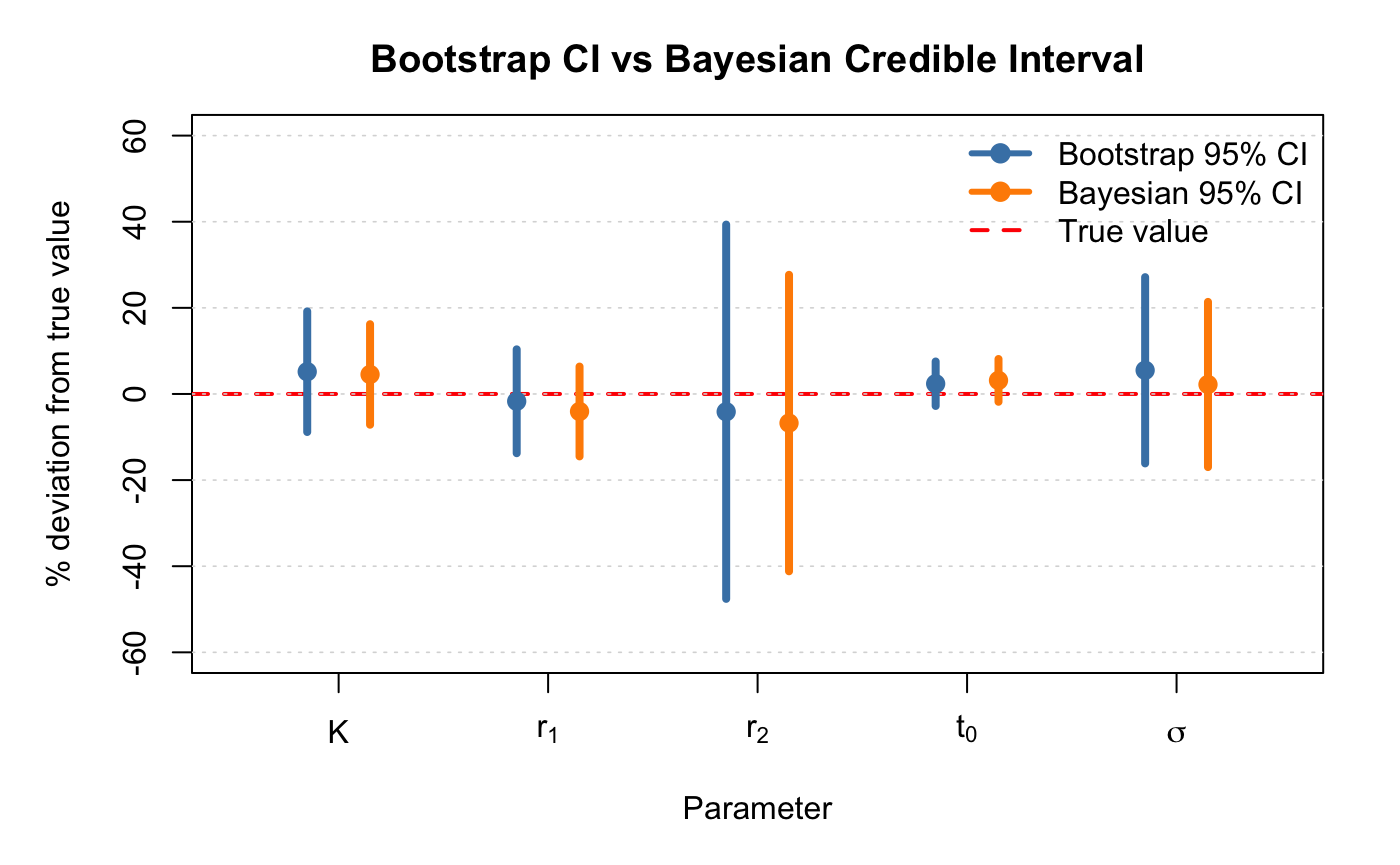
\includegraphics[width=1\linewidth,height=\textheight,keepaspectratio]{ci.png}

}

\caption{Comparison of bootstrap confidence intervals and Bayesian
credible intervals.}

\end{figure}%
\end{column}

\begin{column}{0.45\linewidth}
\begin{itemize}
\tightlist
\item
  Close agreement for all continuous parameters.
\item
  \(\tau\) is estimated precisely by both methods:

  \begin{itemize}
  \tightlist
  \item
    bootstrap \((28,31)\)
  \item
    Bayesian \((30,31)\)
  \end{itemize}
\item
  \(K\) has the largest uncertainty.
\item
  \(r_1\) is estimated more precisely than \(r_2\).
\end{itemize}
\end{column}
\end{columns}
\end{frame}

\begin{frame}{SIR Model}
\phantomsection\label{sir-model}
\begin{itemize}
\tightlist
\item
  Logistic growth captures overall epidemic patterns, but not
  transmission mechanisms.
\item
  We extend the analysis to the \textbf{SIR model}:

  \begin{itemize}
  \tightlist
  \item
    \(S\): susceptible
  \item
    \(I\): infected
  \item
    \(R\): recovered
  \end{itemize}
\item
  Key advantage:

  \begin{itemize}
  \tightlist
  \item
    mechanistic description of disease spread
  \end{itemize}
\item
  Main challenge:

  \begin{itemize}
  \tightlist
  \item
    no closed-form solution
  \item
    must solve an ODE system numerically
  \end{itemize}
\end{itemize}
\end{frame}

\begin{frame}{SIR Change-Point Model}
\phantomsection\label{sir-change-point-model}
\begin{itemize}
\tightlist
\item
  Introduce a change-point in the transmission rate:
\end{itemize}

\[
\beta(t)=
\begin{cases}
\beta_1, & t \le \tau,\\
\beta_2, & t > \tau.
\end{cases}
\]

\begin{itemize}
\tightlist
\item
  Observation model:
\end{itemize}

\[
y_t = I(t;\theta) + \varepsilon_t, \qquad \varepsilon_t \sim N(0,\sigma^2)
\]

\begin{itemize}
\tightlist
\item
  The SIR dynamics are governed by differential equations and solved
  numerically at each evaluation.
\item
  This allows the model to capture interventions or behavioral changes.
\end{itemize}
\end{frame}

\begin{frame}[fragile]{Frequentist Estimation: SIR Model}
\phantomsection\label{frequentist-estimation-sir-model}
\begin{itemize}
\tightlist
\item
  Parameters estimated by MLE
\item
  Equivalent to minimizing the negative log-likelihood
\item
  For a fixed candidate \(\tau\):

  \begin{itemize}
  \tightlist
  \item
    estimate \(\beta_1, \beta_2, \gamma, \sigma\) using \texttt{optim()}
    with \texttt{L-BFGS-B}
  \item
    solve the ODE system numerically at each likelihood evaluation
  \end{itemize}
\item
  Estimate \(\tau\) by grid search over candidate values
\item
  Select the value of \(\tau\) that minimizes the negative
  log-likelihood
\end{itemize}
\end{frame}

\begin{frame}{SIR Simulation Study}
\phantomsection\label{sir-simulation-study}
\begin{itemize}
\tightlist
\item
  Time points: \(t = 0,\dots,60\)
\item
  True parameters:

  \begin{itemize}
  \tightlist
  \item
    \(\beta_1 = 0.40\)
  \item
    \(\beta_2 = 0.15\)
  \item
    \(\gamma = 0.10\)
  \item
    \(\tau = 20\)
  \end{itemize}
\item
  Initial conditions:

  \begin{itemize}
  \tightlist
  \item
    \(S(0) = 0.999\)
  \item
    \(I(0) = 0.001\)
  \item
    \(R(0) = 0\)
  \end{itemize}
\item
  Gaussian noise with \(\sigma = 0.01\)
\item
  Repeat over 100 simulated datasets
\item
  Metrics:

  \begin{itemize}
  \tightlist
  \item
    bias
  \item
    RMSE
  \item
    change-point accuracy
  \end{itemize}
\end{itemize}
\end{frame}

\begin{frame}{SIR Simulation Results}
\phantomsection\label{sir-simulation-results}
\begin{longtable}[]{@{}lrrrr@{}}
\toprule\noalign{}
Parameter & True & Mean Estimate & Bias & RMSE \\
\midrule\noalign{}
\endhead
\(\beta_1\) & 0.40 & 0.4016 & 0.0016 & 0.0093 \\
\(\beta_2\) & 0.15 & 0.1531 & 0.0031 & 0.0230 \\
\(\gamma\) & 0.10 & 0.1004 & 0.0004 & 0.0061 \\
\(\tau\) & 20.00 & 19.84 & -0.16 & 0.5477 \\
\bottomrule\noalign{}
\end{longtable}

\begin{itemize}
\tightlist
\item
  Very small bias across all parameters
\item
  Low RMSE indicates accurate recovery
\item
  \(\beta_2\) shows slightly higher variability because of post-change
  uncertainty
\item
  \(\tau\) is accurately detected
\end{itemize}
\end{frame}

\begin{frame}{Bootstrap Results: SIR Model}
\phantomsection\label{bootstrap-results-sir-model}
\begin{itemize}
\tightlist
\item
  Bootstrap quantifies uncertainty in the SIR parameters
\item
  200 bootstrap replications
\item
  Bootstrap distribution of \(\hat\tau\):

  \begin{itemize}
  \tightlist
  \item
    mean = 19.875
  \item
    SD = 0.6335
  \end{itemize}
\end{itemize}

\begin{longtable}[]{@{}lrr@{}}
\toprule\noalign{}
Parameter & Lower & Upper \\
\midrule\noalign{}
\endhead
\(\beta_1\) & 0.3799 & 0.4186 \\
\(\beta_2\) & 0.1001 & 0.2006 \\
\(\gamma\) & 0.0866 & 0.1110 \\
\(\tau\) & 19.00 & 21.00 \\
\bottomrule\noalign{}
\end{longtable}

\begin{itemize}
\tightlist
\item
  All true values lie within the confidence intervals
\item
  \(\tau\) is estimated with good precision
\item
  \(\beta_2\) shows the widest uncertainty
\end{itemize}
\end{frame}

\begin{frame}{Bayesian SIR Model}
\phantomsection\label{bayesian-sir-model}
\begin{itemize}
\tightlist
\item
  Bayesian inference captures full posterior uncertainty for the
  ODE-based model
\item
  Weakly informative priors over biologically meaningful ranges
\item
  Likelihood requires numerical ODE solving at every MCMC step
\end{itemize}

\textbf{MCMC setup}

\begin{itemize}
\tightlist
\item
  Metropolis-within-Gibbs sampler
\item
  Continuous parameters: Gaussian random walk
\item
  \(\tau\): discrete random walk
\item
  30,000 iterations
\item
  5,000 burn-in
\item
  thinning by 10
\item
  2,500 retained posterior samples
\end{itemize}
\end{frame}

\begin{frame}{Convergence Diagnostics: SIR Model}
\phantomsection\label{convergence-diagnostics-sir-model}
\begin{longtable}[]{@{}lrr@{}}
\toprule\noalign{}
Parameter & Proposal SD & Acceptance Rate \\
\midrule\noalign{}
\endhead
\(\beta_1\) & 0.005 & 0.275 \\
\(\beta_2\) & 0.008 & 0.365 \\
\(\gamma\) & 0.003 & 0.226 \\
\(\sigma\) & 0.005 & 0.182 \\
\(\tau\) & \(\pm\{1,2\}\) & 0.000 \\
\bottomrule\noalign{}
\end{longtable}

\begin{longtable}[]{@{}rrrrl@{}}
\toprule\noalign{}
\(\beta_1\) & \(\beta_2\) & \(\gamma\) & \(\sigma\) & \(\tau\) \\
\midrule\noalign{}
\endhead
\(\sim 150\) & \(\sim 100\) & \(\sim 120\) & \(\sim 1200\) & 0 (point
mass) \\
\bottomrule\noalign{}
\end{longtable}

\begin{itemize}
\tightlist
\item
  Continuous parameters have acceptable mixing.
\item
  \(\tau\) has zero acceptance, not because of sampler failure, but
  because the posterior collapses at the true value.
\item
  \(\sigma\) mixes very efficiently; \(\beta_1, \beta_2, \gamma\) show
  moderate dependence due to the shared ODE structure.
\end{itemize}
\end{frame}

\begin{frame}{Posterior Summary: SIR Model}
\phantomsection\label{posterior-summary-sir-model}
\begin{longtable}[]{@{}lrrrl@{}}
\toprule\noalign{}
Parameter & True & Mean & Median & 95\% CI \\
\midrule\noalign{}
\endhead
\(\beta_1\) & 0.40 & 0.4060 & 0.4060 & \((0.4006, 0.4110)\) \\
\(\beta_2\) & 0.15 & 0.1707 & 0.1706 & \((0.1495, 0.1908)\) \\
\(\gamma\) & 0.10 & 0.1054 & 0.1053 & \((0.0996, 0.1106)\) \\
\(\sigma\) & 0.01 & 0.0093 & 0.0092 & \((0.0078, 0.0112)\) \\
\(\tau\) & 20 & point mass & & \(\tau=20\) \\
\bottomrule\noalign{}
\end{longtable}

\begin{itemize}
\tightlist
\item
  Posterior inference recovers the true parameters well.
\item
  \(\sigma\) is the most precisely estimated.
\item
  \(\beta_2\) has the largest uncertainty.
\item
  \(\tau\) is point-identified at the true value.
\end{itemize}
\end{frame}

\begin{frame}{SIR: Posterior Fit and Interpretation}
\phantomsection\label{sir-posterior-fit-and-interpretation}
\begin{columns}[T]
\begin{column}{0.58\linewidth}
\begin{figure}[H]

{\centering 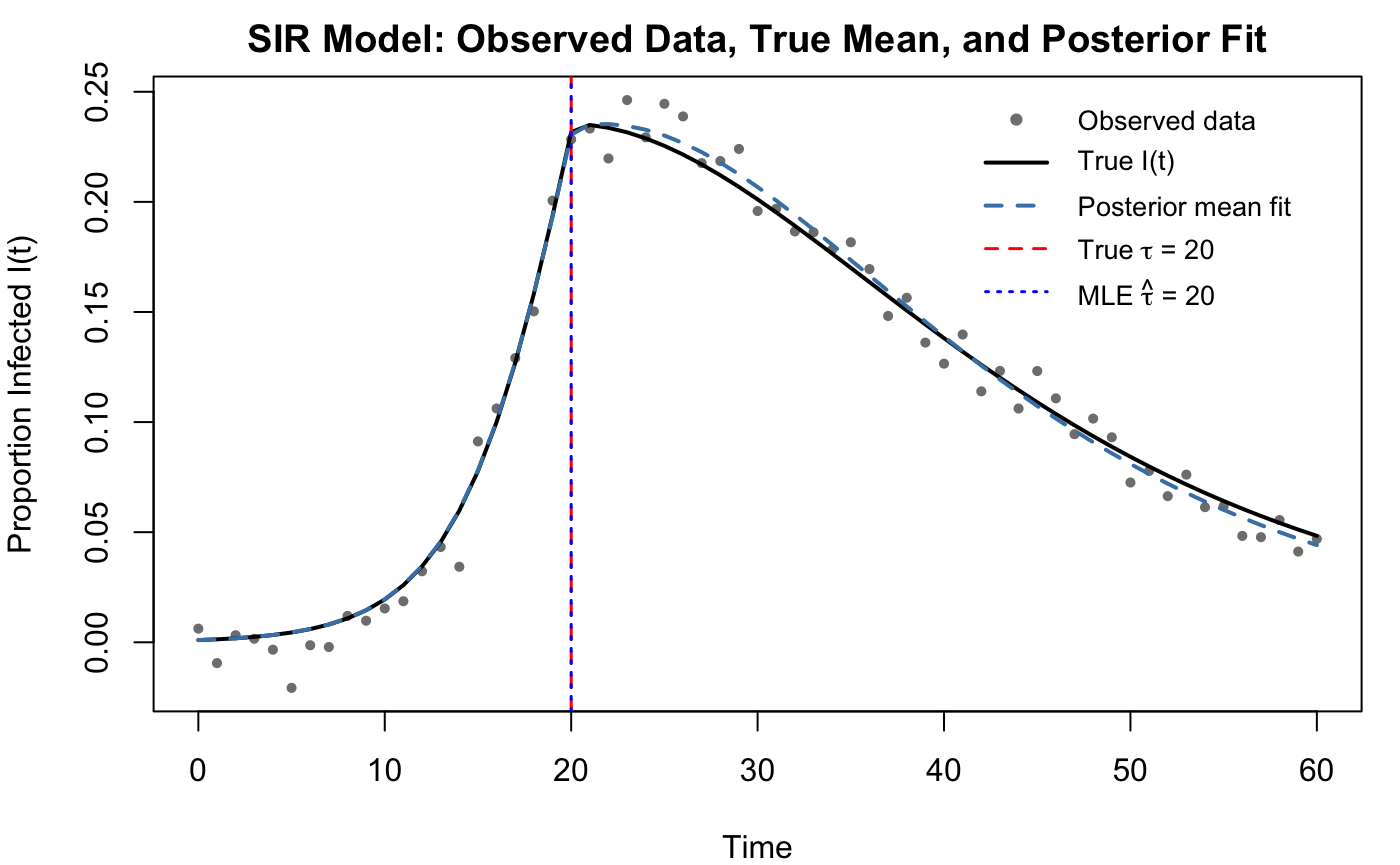
\includegraphics[width=1\linewidth,height=\textheight,keepaspectratio]{SIR.png}

}

\caption{SIR model fitted trajectory.}

\end{figure}%
\end{column}

\begin{column}{0.42\linewidth}
\begin{itemize}
\tightlist
\item
  Posterior fit closely matches the observed epidemic curve.
\item
  The change-point is correctly identified at \(\tau = 20\).
\item
  The model captures both the epidemic peak and the post-intervention
  decline.
\item
  This supports stronger change-point identifiability in the SIR model
  than in the logistic model.
\end{itemize}
\end{column}
\end{columns}
\end{frame}

\begin{frame}{Bootstrap vs Bayesian: SIR Model}
\phantomsection\label{bootstrap-vs-bayesian-sir-model}
\begin{longtable}[]{@{}lll@{}}
\toprule\noalign{}
Parameter & Bootstrap CI & Bayesian CI \\
\midrule\noalign{}
\endhead
\(\beta_1\) & \((0.3799, 0.4186)\) & \((0.4006, 0.4110)\) \\
\(\beta_2\) & \((0.1001, 0.2006)\) & \((0.1495, 0.1908)\) \\
\(\gamma\) & \((0.0866, 0.1110)\) & \((0.0996, 0.1106)\) \\
\bottomrule\noalign{}
\end{longtable}

\begin{itemize}
\tightlist
\item
  Strong agreement for \(\beta_1\)
\item
  Wider Bayesian interval for \(\beta_2\)
\item
  Slight differences reflect stronger posterior dependence in the SIR
  model
\item
  Both methods support the same qualitative conclusions
\end{itemize}
\end{frame}

\begin{frame}{Computational Considerations}
\phantomsection\label{computational-considerations}
\begin{itemize}
\tightlist
\item
  Strong computational contrast between logistic and SIR models
\end{itemize}

\textbf{Logistic model}

\begin{itemize}
\tightlist
\item
  closed-form mean function
\item
  fast likelihood evaluation
\item
  efficient profile search
\end{itemize}

\textbf{SIR model}

\begin{itemize}
\tightlist
\item
  requires numerical ODE solution at each evaluation
\item
  much slower profile likelihood and MCMC
\item
  repeated ODE solves dominate runtime
\end{itemize}

\textbf{Implication:} model realism improves, but computational cost
increases sharply.
\end{frame}

\begin{frame}[fragile]{Numerical Stability and Initialization}
\phantomsection\label{numerical-stability-and-initialization}
\textbf{Logistic model}

\begin{itemize}
\tightlist
\item
  stable optimization across simulations
\item
  smooth likelihood surface
\item
  reliable convergence with \texttt{L-BFGS-B}
\end{itemize}

\textbf{SIR model}

\begin{itemize}
\tightlist
\item
  requires ODE solver safeguards
\item
  occasional instability for extreme parameter values
\item
  stability improves with safe evaluation wrappers
\end{itemize}

\textbf{Initialization}

\begin{itemize}
\tightlist
\item
  MLE estimates used as starting values for MCMC
\item
  low sensitivity for logistic model
\item
  stronger sensitivity for SIR model
\item
  MLE initialization improves convergence and reduces burn-in
\end{itemize}
\end{frame}

\begin{frame}{Change-Point Identifiability}
\phantomsection\label{change-point-identifiability}
\textbf{Logistic model}

\begin{itemize}
\tightlist
\item
  \(\tau\) moves between nearby values 30 and 31
\item
  indicates moderate uncertainty
\end{itemize}

\textbf{SIR model}

\begin{itemize}
\tightlist
\item
  \(\tau\) remains fixed at 20
\item
  indicates extreme identifiability
\end{itemize}

\textbf{Interpretation}

\begin{itemize}
\tightlist
\item
  the SIR likelihood is much more sensitive to the change-point
\item
  incorrect values are strongly penalized
\item
  more mechanistic models can produce stronger change-point
  detectability
\end{itemize}
\end{frame}

\section{Summarry}\label{summarry}

\begin{frame}{Practical Recommendations}
\phantomsection\label{practical-recommendations}
\begin{itemize}
\tightlist
\item
  \textbf{Model selection:} AIC works well for choosing between
  no-change and change-point models
\item
  \textbf{Change-point estimation:} profile likelihood grid search is
  efficient and interpretable
\item
  \textbf{Uncertainty quantification:} both bootstrap and Bayesian
  methods are valid
\item
  \textbf{Computational caution:} bootstrap is much more expensive for
  ODE-based models
\item
  \textbf{MCMC practice:}

  \begin{itemize}
  \tightlist
  \item
    initialize at MLEs
  \item
    tune continuous-parameter acceptance rates to \(0.20\)--\(0.50\)
  \item
    zero acceptance for a discrete parameter can indicate strong
    identifiability rather than failure
  \end{itemize}
\end{itemize}
\end{frame}

\begin{frame}{Discussion and Conclusion}
\phantomsection\label{discussion-and-conclusion}
\begin{itemize}
\tightlist
\item
  Both logistic and SIR change-point models recover parameters
  accurately.
\item
  Logistic model:

  \begin{itemize}
  \tightlist
  \item
    simpler
  \item
    faster
  \item
    less computationally expensive
  \end{itemize}
\item
  SIR model:

  \begin{itemize}
  \tightlist
  \item
    more realistic
  \item
    computationally intensive
  \item
    yields stronger change-point identifiability
  \end{itemize}
\item
  Frequentist and Bayesian methods agree strongly in the logistic model
  and remain broadly consistent in the SIR model.
\item
  Main conclusion:

  \begin{itemize}
  \tightlist
  \item
    model structure strongly affects identifiability, computational
    cost, and uncertainty quantification
  \end{itemize}
\end{itemize}
\end{frame}

\begin{frame}{Thank you}
\phantomsection\label{thank-you}
\begin{center}
\Large Thank you\\[0.5em]
\large Questions?
\end{center}
\end{frame}




\end{document}
